\section{Method}


First, we will define an function that is uniquely minimized by unitary matrices and some favorable properties for optimization.
This will be the ground truth we evaluate the success of our method against.
We then define the multitask lasso method that approximates the ground truth loss function in the sense that loss values are the same for all diagonalizable matrices.
We show that this program recovers to optimum in a deterministic manner should it exist, but that the solution is not necessarily $D-sparse$.
Therefore, we will demonstrate the ways in which sparse 
% NOTE (Sam): we have not yet shown that the optimum is always D sparse if it exists...

\subsection{Ground truth}

The main goal of sparse isometry pursuit is to expediate the selection of unitary submatrices.
Typical measures of unitariness which use the singular values of a matrix like the operator norm (i.e. deformation) and nuclear norm are poorly suited for  optimization since they use a subset of the matrix's information and are not uniquely minimized at unitarity, respectively.

% NOTE (Sam): %is our the convex dual of itself?

Define the loss
\begin{align}
l_{iso}: \mathbb R^{D \times P} \to \mathbb R^{+} \\
\mathcal (X) \mapsto \sum_{d = 1}^D g(\sigma^d(\mathcal X))
\end{align}
where $\sigma^d (\mathcal (X))$ is the $d$-th singular value of $\mathcal X$.
%Note that since $g$ is convex, we could compute a full realization of the convex isometry pursuit algorithm by minimizing over WHAT.
However, this would not result in a sparse solution.

This loss is an appropriate choice for comparison because it is equal to the basis pursuit loss for suitably normalized orthogonal matrices.
This will be discussed


\subsection{Normalization}
% NOTE (Sam): balance goes out the window with great flowers since there is no normalization.

% NOTE (Sam): it might be nice to borrow the normalization, optimization, and postprocessing step lexicon from the neuroscience paper.
Since basis pursuit methods tend to select longer vectors, selection of unitary submatrices requires normalization such that long and short candidate basis vectors are penalized in the subsequent regression.
This calls for a "normalization" method that differs from other forms in its requirements, and we can't yet prove that these conditions relate it to any sort of norm on an appropriately chosen space.
However, this transformation of individual features should be familiar to statisticians as a form of feature engineering, and whether the transformed vectors are related to a norm or not, the concept is similar.

We may now establish some basic conditions for normalization of vectors $v \in \mathbb R^D$.

\begin{definition}[Symmetric normalization]
A function $q: \mathbb R^D \to \mathbb R^+ $ is a symmetric normalization if 
\begin{align}
\arg \max_{v \in \mathbb R^D} \ q (v) &=\{ v \; \|v\| = 1 \} \\
q(v) &= q(\frac{v}{\|v\|^2}) \\
q(v^1) &= q(v^2) \; \forall v^1, v^2 : \|v^1\| = \|v^2\|
\end{align}
\label{cond:normalization}
\end{definition}

Note that requiring the full structure of a multiplicative norm here is unnecessary for basic success of the algorithm, but certain characteristics such as $q(v^{-1}) = q(v)$ seem desirable, provided one can give a reasonable way to compute $v^{-1}$, such as by considering each vector as a scaled rotation subgroup of the general linear group.
Mindful of this opportunity, and also of the desire to compare with the ground truth and provide computational expediency, consider the normalization by
\begin{align}
\label{eq:normalization}
% Note (Sam): fix this... get and more ... q_c?
q: \mathbb R^+ \times \mathbb R^+  &\to \mathbb R^+ \\
t , c &\mapsto \frac{\exp(t^c) + \exp(t^{-c})}{2e},
\end{align}
and use this to define the normalization 
\begin{align}
n: \mathbb R^D \times \mathbb R^+ &\to \mathbb R^D \\
n^d , c &\mapsto \frac{n^d}{q(\|n\|_{2},c) } \forall d \in [D].
\end{align}

While this normalization satisfies \ref{cond:normalization}, it also has some additional nice properties.
First, $q$ is convex and smooth.
Second, it grows asymptotically log-linearly.
Third, while $\exp(-|\log t|) = \exp(-\max (t, 1/t))$ is a seemingly natural choice for normalization, it is non smooth, and the LogSumExp replacement of $\max (t, 1/t)$ with $ \log (\exp (t ) + \exp(1/t))$ simplifies to \ref{eq:normalization} upon exponentiation.
% Introduce the exponent here.
Finally, the parameter $c$ grants control over the width of the basin, which is important in avoiding numerical issues arising close to $0$ and $\infty$.

\begin{figure}[htbp]
    \centering
    \begin{minipage}{0.49\textwidth}
        \centering
        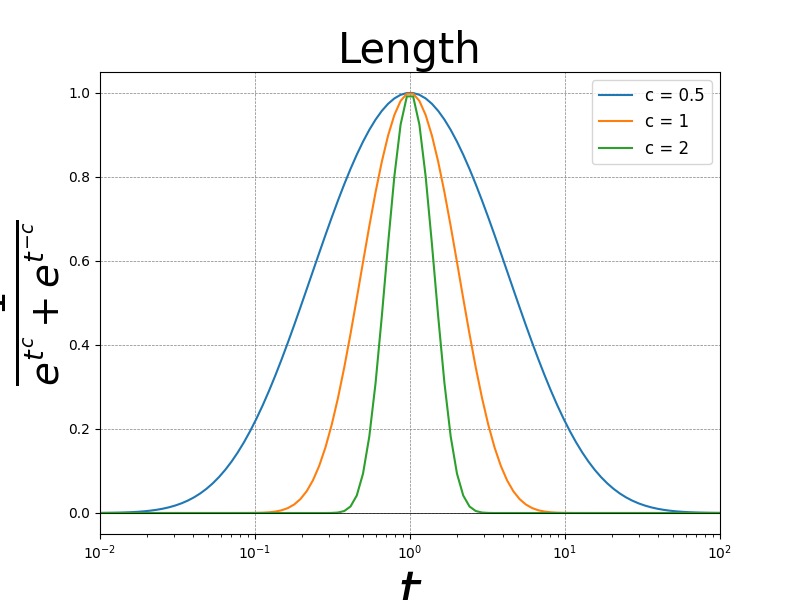
\includegraphics[width=\textwidth]{../figures/Figure_1a.png}
        \caption{Length as a function of $t$}
        \label{fig:length}
    \end{minipage}
    \hfill
    \begin{minipage}{0.49\textwidth}
        \centering
        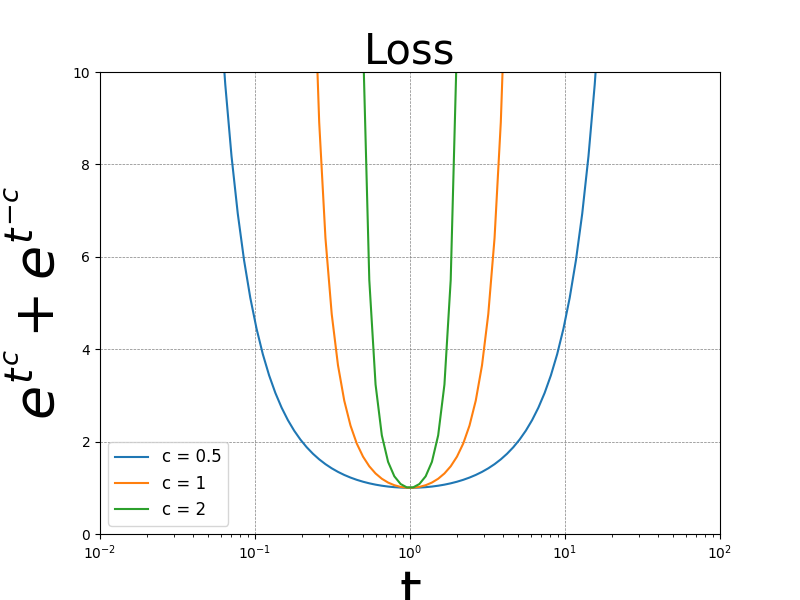
\includegraphics[width=\textwidth]{../figures/Figure_1b.png}
        \caption{Loss as a function of $t$}
        \label{fig:loss}
    \end{minipage}
    \caption{Plots of Length and Loss for different values of $c$.
    Since $t$ is one dimensional and therefore diagonalizable, basis pursuit and ground truth give identical loss values.}
    \label{fig:results}
\end{figure}


Using this, define the matrix-wide normalization vector
\begin{align}
\mathcal D: \mathbb R^{D \times P} \times \mathbb R^+ &\to \mathbb R^P \\
\mathcal X_{.p}, c &\mapsto n(\mathcal X_{.p}, c)
\end{align}
and the normalized matrix $\tilde {\mathcal X}_c = \mathcal X \mathcal D(\mathcal X, c).$
This completes the data preprocessing.



\subsection{Isometry pursuit}

Define the multitask group basis pursuit penalty % is this really a norm?
\begin{align}
\label{eq:bp}
\| \cdot \|_{1,2}: \mathbb R^{P \times D} &\to \mathbb R^+ \\ 
\beta &\mapsto  \sum_{p=1}^P  \|\beta_{p.}\|_2.
\end{align}

The isometry pursuit program is then
\begin{align}
\label{prog:isometry_pursuit}
\hat {\beta_{P}} (\mathcal X)  = \arg \min_{\beta \in \mathbb R^{P \times D}} \| \beta \|_{1,2} \; s.t. \; I_D = \tilde{ \mathcal X}_c \beta.
\end{align}
The intuition is that vectors which are closer to 1 in length and more orthogonal will be smaller in loss.

%Direct minimization of Equation \ref{eq:bp} will not select for isometry due to the preference for columns with larger norm.

%One immediate question is - why $\beta$?  Can we just minimize some function of $X$ directly like $\|\exp_1 X\|_{1,2}$?  Direct minimization of this norm has nothing to do with correlation. We wouldn't need orthogonality - just constant length!

\subsection{Isometric lasso}

The convex loss function \ref{eq:bp} and linear constraint in \ref{prog:isometry_pursuit} admit a Lagrangian dual which we shall call Isometric Lasso.
The Isometric Lasso loss is
\begin{align}
l_\lambda (\mathcal X, \beta) =  \|I_D -  \tilde{ \mathcal X}_c \beta\|_2^2 +  \lambda \| \beta \|_{1,2}
\end{align}
which can be optimized as
\begin{align}
\label{prog:isometric_lasso}
\hat {\beta_{\lambda}} (\mathcal X) = \arg \min_{\beta \in \mathbb R^{P \times D}} l_\lambda (\mathcal X, \beta)
\end{align}
The recovered supports are then given by $S(\hat {\beta_{\lambda}} (\mathcal X))$ where 
\begin{align}
S: \mathbb{R}^{p \times d} &\to \binom{\{1, 2, \ldots, P\}}{d} \\
\beta &\mapsto \left\{ p \in \{1, 2, \ldots, P\} :  \|\beta_{p.}\| > 0 \right\}
\end{align}
and $\binom{\{1, 2, \ldots, P\}}{d} = \left\{ A \subseteq \{1, 2, \ldots, P\} : \left|A\right| = d \right\}$ are the indices of the dictionary elements with non-zero coefficients.

\subsection{Theory}
\label{sec:theory}

A key theoretical assertion is that selection methods $S(\widehat {\beta}_{\lambda} (\mathcal X))$ and $S(\widehat {\beta} (\mathcal X))$ are invariant to choice of basis for $\mathcal X$.

\begin{proposition}[Basis pursuit selection equivalence]
\label{prop:basis_pursuit_selection_equivalence}
Let $U \in \mathbb R^{D \times D}$ be unitary.
 Then $S(\widehat \beta  (U \mathcal X)) = S(\widehat \beta (\mathcal X))$.
\end{proposition}

\begin{proposition}[Lasso selection equivalence]
\label{prop:lasso_selection_equivalence}
Let $U \in \mathbb R^{D \times D}$ be unitary.
 Then $S(\widehat \beta_{\lambda}  (U \mathcal X)) = S(\widehat \beta_{\lambda} (\mathcal X))$.
\end{proposition}

%It also may be possible to argue the basis pursuit invariance from the lasso ones plus Lagranian duality, but to avoid taking the limit we prove both propositions  independently.
%This also covers changing the target variable.

With these preliminaries, we may state our main result.

\begin{proposition}[Unitary selection]
\label{prop:unitary_selection}
Given a matrix $\mathcal X \in \mathbb R^{D \times P}$ with a rank $D$ submatrix $\mathcal X_{.\mathcal S} \in \mathbb R^{D \times D}$ that is unitary, $\mathcal S = S(\widehat{\beta} (\mathcal X)))$
%Program \ref{prog:isometry_pursuit} selects $\mathcal S \subset [P]$ with $|\mathcal S| = D$ such that $X_{. \mathcal S}$
 \end{proposition}
 
 A proof is given in Section 
 
This proof admits two immediate generalizations.
First, any normalization function that satisfies the normalization conditions will do.
Second, the ground truth and convex losses are equivalent for diagonalizable matrices.


\begin{proposition}
\label{prop:main}
\end{proposition}
\begin{proof}
\begin{align}
\end{align}
Then, singular values and regressands are analytically determined.  cont.
\end{proof}


 %Convex functions form metric? Cite Koelle neuroscience? Is metric important?
 
\begin{proposition}[Local isometry selection]
\label{prop:local_isometry}
Given a set of functions $G$ that contains a subset that defines a locally isometric embedding at a point $\xi$, then these will be selected as $\arg \min_\beta$.
\end{proposition}
A proof is given in Section \ref{sec:local_isometry_proof}.


Algorithm (Local tangent Space basis pursuit)

Algorithm (Local two stage tangent space basis pursuit)

This provides an approach for the problem put forward in (cite) LDLE paper.

Experiments (Loss)

Compare with isometry loss (2 norm of singular values).

\subsection{Implementation}

We use the multitask lasso from sklearn and the cvxpy package for basis pursuit.  We use the SCS interior point solver from CVXPY, which is able to push sparse values arbitrarily close to 0 \cite{cvxpy_sparse_solution}. Data is IRIS and Wine, as well as flat torus from ldle.
\subsection{Computational complexity}
\section{Experiments}

Comparison with isometry loss.